\documentclass[twocolumn]{svjour3}[2016]

\usepackage{graphicx}
\usepackage{cite}
\usepackage{subfig}
\usepackage{mathtools}
\usepackage{amsmath}
\usepackage{amssymb}

\begin{document}
%HEADER
\title{Exploring Unstructured Environment with Frontier Trees}
\author{R. Korb \and A. Schoettl}
\institute{
	Rudolf F. S. Korb \at
	University of Applied Sciences - Munich\\ Dept. 04 Electrical Engineering and Information Technology, Laboratory for Autonomous Systems in Munich (LASIM),  Lothstr. 64, 80335 Munich, Germany\\Tel.: +49-89-1265-3415\\
	\email{rudolf.korb@hm.edu}
	\and
	Alfred Schoettl \at
	University of Applied Sciences - Munich\\ Dept. 04 Electrical Engineering and Information Technology, Laboratory for Autonomous Systems in Munich (LASIM),  Lothstr. 64, 80335 Munich, Germany\\Tel.: +49-89-1265-3415\\
	\email{alfred.schoettl@hm.edu}
}

\maketitle

\begin{abstract}
\textbf{
%\textit{
	This paper presents the Frontier Tree exploration algorithm, a novel approach to autonomously explore unknown and unstructured areas. Focus of this work is the exploration of domestic environments with arbitrary obstacles, for example furbished appartements. Existing and well studied approaches like greedy algorithms perform worse, when obstacles are included and the range of distance sensors is limited. Base of this research is the Frontier Tree. This data structure offers two main features. It is a memory of past poses during exploration and is utilized to decide between future navigation goals. This approach is compared to a basic but efficient nearest neighbour exploration. The algorithm is tested in simulation with maps similar to appartement ground maps including furniture as obstacles. The paper shows, that frontier trees minimize the travelled path of the mobile robot by tracking open boundaries.

}
\keywords{Robotics \and  Exploration \and  Path Planning \and  Frontiers \and Domestic Environment}
\end{abstract}

\section{Introduction}
\label{introduction}
Mobile robots must be familiar with their surroundings to execute complex tasks, for example pick-up and delivery services. As an initial step, the workspace has to be explored autonomously. This problem can be divided into three parts; mapping, localization and exploration. Focus of this research is planning future exploration steps to uncover the environment efficiently, depending on past steps, a map of the area already explored and the agent's current position.\\
When robots participate in everyday life, their operation space consists of unstructured, dynamic environments and has to deal with interieur and crowded areas.
As a consequence, when service robots operate in private appartements or public buildings like hospitals or retirement homes, they need to adapt itselves to their surroudings.
Therefore it is crucial for a mobile robot to explore areas autonomously and not rely on an environment designed specifically for a service device.\\
Basic algorithms follow a greedy approach to select future robot positions during the exploration problem. These approaches use the robot's current state and plan one step ahead by minimizing a cost function, for example the agent's euclidian distance to a boundary of known and unknown space. For exploration of simple maps, unfurbished rooms and corridors, basic algorithms provide acceptable results, depending on for example sensor constraints. With high range distance sensors and obstacle free areas, robots cover the entire room before leaving and most likely do not create open boundaries. Therefore, rooms do not have to be visited again and the traveled distance is less compared to low range sensing robots. Furthermore, the number of possible decisions to choose the next goal from is rising with the environment's complexity. As a result, the greedy algorithm's performance will decrease. The robot has to revisit parts of the map where boundaries have been forgotten, increasing the traveled distance.\\
Consequently the two main influences for travelling distance during exploration is the complexity of an agent's environment and constraints of its range sensors. Mobile autonomous robots in unstructered environment are dealing with both, high complexity and sensor limitations. Many algorithms use maps with reduced difficulty, expecting an empty environment or assume a sensor with infinite distance measurements. It follows, that algorithms covering only one impact decrease in efficiency, when a complex environment and sensor limitations are present.\\
Greedy algorithms dealing with both influences have one major flaw, which leads to a rise of traveled distance and exploration time. Approaching a boundary already discovered several steps ahead, is an indication that the robot's current exploration path is a cycle. As a result, open boundaries between the starting and endpoint of the cycle will be reached with high travel costs later on during the exploration task. The frontier tree recognizes cycles and hence is able to avoid high costs and react early on forgotten boundaries.

% For one-column wide figures use
%\begin{figure}
%  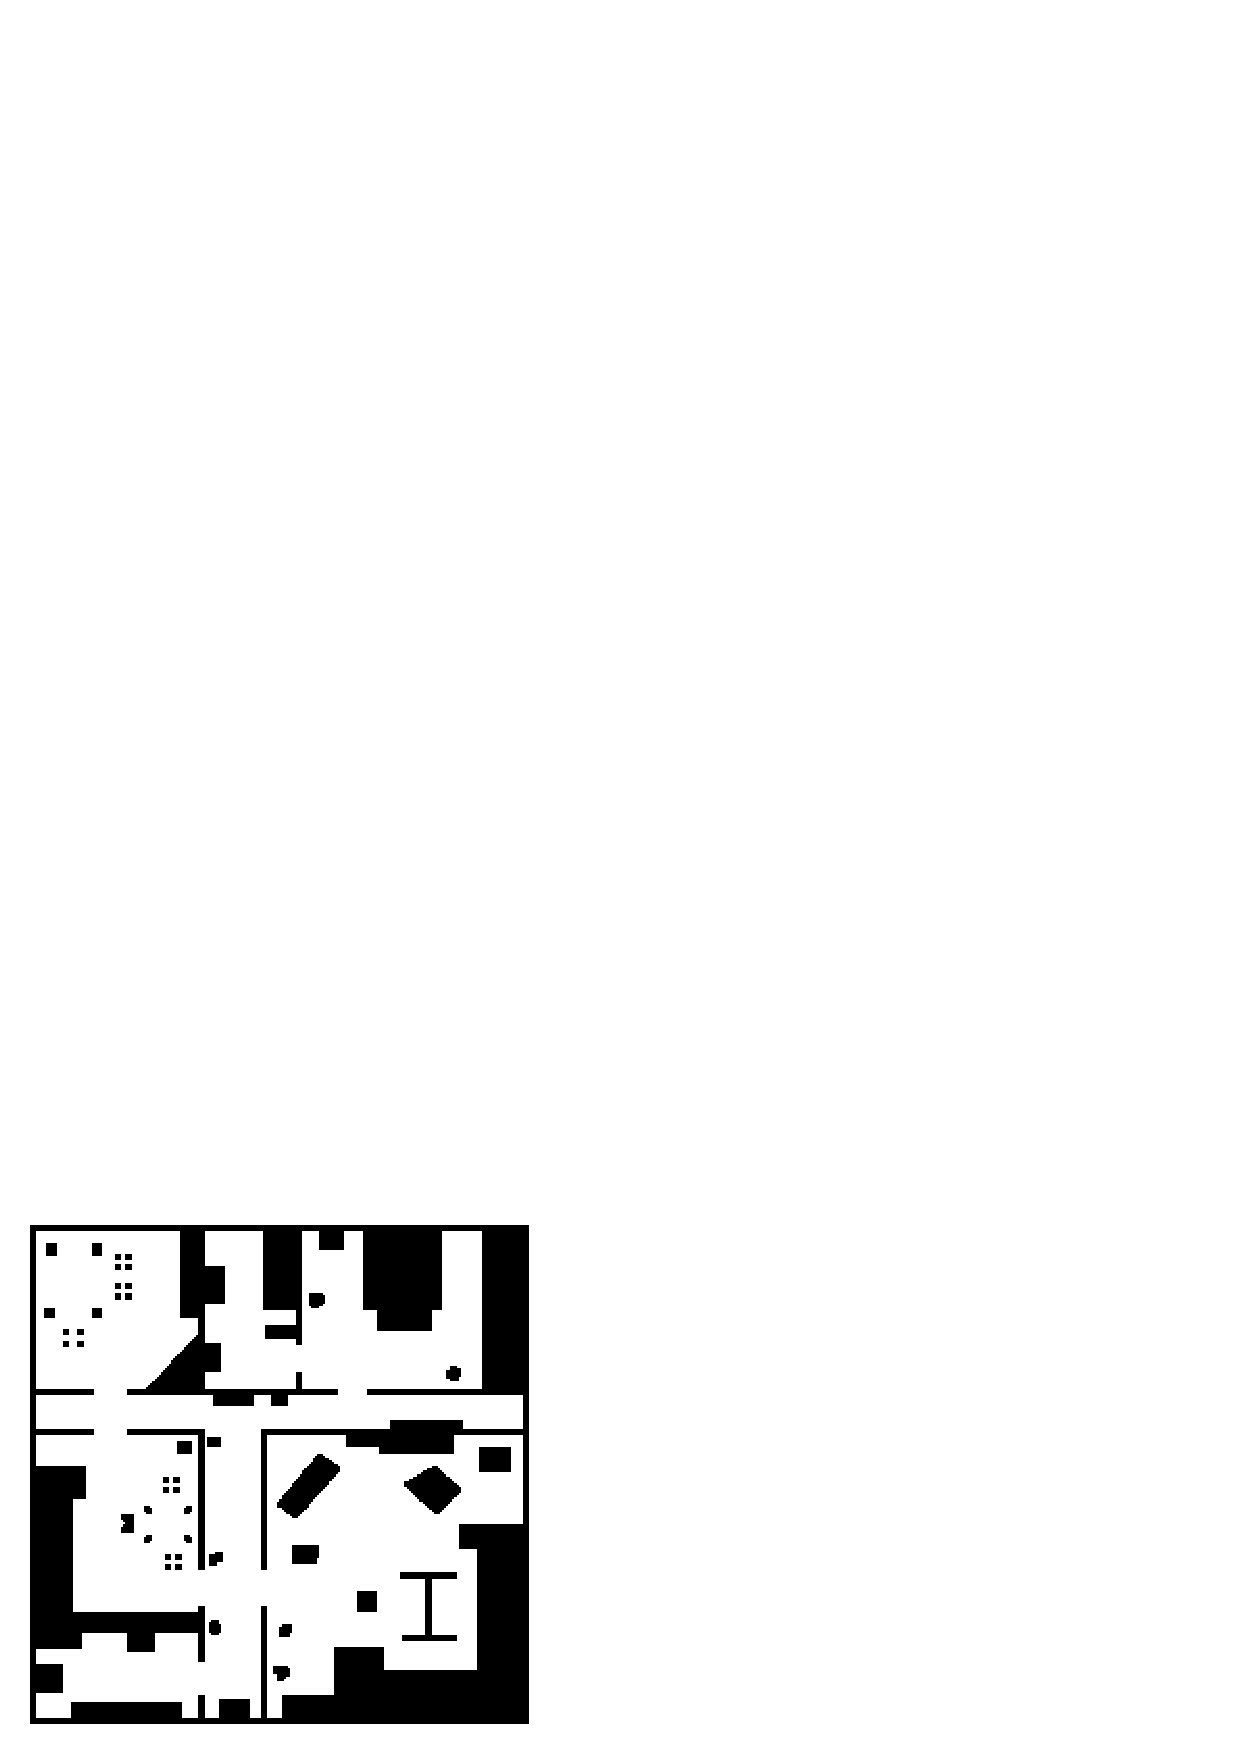
\includegraphics[width=5cm,height=5cm]{map_19.pdf}
% figure caption is below the figure
%\caption{Please write your figure caption here}
%\label{fig:1}       % Give a unique label
%\end{figure}

\section{Related Work}
\label{related_work}
Many exploration algorithms use the frontier approach introduced by Yamauchi \cite{brian_yamauchi_frontier-based_2007}. A frontier is defined as the boudary between known and unknown space in the currently explored map. The algorithm proposed in this paper also utilizes frontiers as atomic elements in the tree data structure and are discussed in detail in section \ref{frontiers}. Yamauchi's exploration algorithm is a greedy approch and chooses the shortest obstacle free path to minimize the distance between a robot's position and the next frontier.\\
Koenig et al. \cite{sven_koenig_greedy_2001} show, that greedy algorithms explore ares with acceptable results. For improvements, map segmentation algorithms were introduced \cite{dirk_holz_evaluating_2010, kai_m._wurm_coordinated_2008} to reduce the travel distance of greedy approaches. Wurm et al. \cite{kai_m._wurm_coordinated_2008} use Voronoi Graphs to divide the explored environment in segments. While large emtpy spaces are segmented well, narrow areas, for example corridors, yield a vast amount of partitions. As a result, the disadvantage of greedy algorithms remains. Holz et al. \cite{dirk_holz_evaluating_2010} extend the segmentation by adding a step for merging several partitions.\\
To keep track of open boundaries, Nasir and Elnagar \cite{reem_nasir_gap_2015} use a data structure called Gap Navigation Tree, introduced by Tovar et al. \cite{benjamin_tovar_optimal_2003}.\\
Another approach is using information based heuristics \cite{arnoud_visser_balancing_2008,amir_mobarhani_histogram_2011,robert_grabowski_autonomous_2003}. Visser and Slamet \cite{arnoud_visser_balancing_2008} minimize information entropy by selecting frontiers with the largest area. Additionally, they consider travel distance to each frontier in their cost function, to increase the algoritm's efficiency. In \cite{amir_mobarhani_histogram_2011}, Mobarhani et al. also discuss the tradeoff between an information based heuristic and travel distance. They count the number of points of all frontiers at an angle interval from the robot's current position and fill an angle histogram. The next best frontier is selected with a weighted cost funtion by maximising the number of frontier cells at a specific direction and minimizing the travel time to the frontier.\\
Information based approaches are especially good for rescue scenarios.Focus of these algorithms is uncovering large parts of the map quickly. It is possible that these heuristics result in alternating poses between opposite parts of the map. This behaviour leads to an increased travel distance.\\
%Exploration by a team of mobile robots is also investigated intensively \cite{antonio_franchi_sensor-based_2009,andreas_nuchter_enhanced_2015,cyrill_stachniss_efficient_2008,kai_m._wurm_coordinated_2008,robert_grabowski_autonomous_2003} but is not part of the research in this paper.

\section{Outline}
%The worst case of greedy algorithms is not optimal, but the difference to the worst case optimal travel distance is reasonable small.
Although the difference to between the worst case of greedy algorithms and the worst case optimal travel distance is reasonable small, the performance is reduced with rising map complexity and sensor limitations.
A major weakness of an efficient greedy algorithm is illustrated in figure \ref{fig:1}. When entering a room with obstacles, it is possible, that the robot runs in a cycle and returns to a previous area before finishing the room. This behaviour results in higher travel cost, because the robt has to revisit the room. Segmentation approaches \cite{dirk_holz_evaluating_2010, kai_m._wurm_coordinated_2008} to further reduce travel cost, highly rely on the geometrical appearence of the map. With an environment containing obstacles, the probability of revisiting a room is increasing. Segmentation in combination with merging minimizes the number of segments, but does not eliminate the problem, where the robot's path is in a cycle.\\
With Gap Navigation Trees Tovar et al. \cite{benjamin_tovar_optimal_2003} solve the problem of map complexity with arbitrary obstacles, but assume infinite distance measurement und $360^{\circ}$ opening angle and therefore do not have sensor constraints. A reduced map size grants this property for real life experiments.\\
The exploration algorithm proposed in this paper performs well with complex structure and sensor limitations. It offers the ability to react, when the agent runs in a cycle to prevent further travel cost.

\begin{figure}
  \includegraphics{figures/fig1.pdf}
% figure caption is below the figure
  \caption{
  This illustration shows six robot states during exploration, following a greedy algorithm. The robot enters a room with obstacles and leaves before uncovering the whole area. As a result, the agent has to return at a later exploration step.}
  \label{fig:1}       % Give a unique label
\end{figure}

%Another approach is adding a second cost function to the exlporation algorithm \cite{arnoud_visser_balancing_2008}.
\section{The Frontier Tree Algorithm}
\label{tfta}

Foundation of this exploration algorithm is a tree data structure with frontiers as nodes. The definition of a frontier is related to Yamauchi's approach \cite{brian_yamauchi_frontier-based_2007}. Similar to Gap Navigation Trees \cite{benjamin_tovar_optimal_2003}, the data structure is, inter alia, used for tracking open boundaries during exploration. Additionally, the resulting topological tree map is used to select the next exploration goal. The final path planning to the new pose is executed on a 2D grid map.


\subsection{Robot Model}
In this paper the robot is implemented as mobile base with a circular footprint and three degrees of freedom. The position and orientation is defined by $\textbf{r} = (x, y, \theta)^{T}$ with $x, y$ as position and $\theta$ as orientation. Additionally, the agent provides a distance sensor, represented by $\textbf{s} = (d, \alpha)^{T}$. Component $d$ is the sensor's range and $\alpha$ its opening angle. As an assumption, the robot is able to localize itself on a 2D grid map using a simultaneous localization and mapping (SLAM) approach.

\subsection{Map Representations}
To fulfill the exploration task, the algorithm uses five maps of three different types. A basic map type is the occupancy grid map with values between $0$ and $1$, where white pixels ($1$) mark free and black pixels ($0$) unpassable space. Values in the interval $(0,1)$ can be interpreted as unknown space. An oocupancy map is the output of a SLAM algorithm. Unpassable pixels are inflated by the radius of the robot's footprint, resulting in a global occupancy map $\textrm{occ}_g$ where the agent can be treated as a point. $\textrm{occ}_g$ is used to create a local (with dependency of $\textbf{r}$) occupancy map $\textrm{occ}_{l}$.
\begin{equation}
%\[
\textrm{occ}_ {l}(\textbf{x})=
\begin{dcases}
0.5, & \text{if } \textrm{dist}(\textbf{x}, \textbf{r}) \geq l\\
\textrm{occ}_{g}(\textbf{x}), & \text{otherwise}
\end{dcases}
%\]
\end{equation}
where $\textrm{dist}(\textbf{x}, \textbf{r})$ is the euclidian distance between the considered pixel $\textbf{x}$ in $\textrm{occ}_{local}$ to the current robot position $\textbf{r}$.
\\
Both, $\textrm{occ}_{g}$ and $\textrm{occ}_{l}$, as well as the current pose $\textbf{r}$ are utilized for the calculation of global and local cost maps $\textrm{cost}_{g}$ and $\textrm{cost}_{l}$. These are calculated with Dijstra's Algorithm. Without a return criterion, the result is a map with the $\textrm{cost}(\textbf{x})$ to travel from $\textbf{r}$ to $\textbf{x}$.\\
Lastly, $\textrm{occ}_g$ is used to create a frontier map $\digamma$, containing the possible future goals for exploration. Since $\textrm{occ}_g$ is an inflated representation, every point in $\digamma$ is a possible navigation goal. Section \ref{frontiers} gives a formal description of frontiers.

\begin{figure}
\centering
  \mbox{
  \subfloat[Occupancy map]{
    %\includegraphics{figures/fig2a.pdf}
    \includegraphics[width=39mm]{figures/occupancy_map_13.png}
    \label{fig2:a}
  }
  \subfloat[Frontier map]{
      %\includegraphics{figures/39.pdf}
      \includegraphics[width=39mm]{figures/frontier_map_13.png}
      \label{fig2:b}
    }
  }
    \mbox{
    \subfloat[Cost map]{
      %\includegraphics{figures/fig2c.pdf}
      \includegraphics[width=39mm]{figures/rmap_14.png}
      \label{fig2:c}
    }
    \subfloat[Local cost Map]{
        %\includegraphics{figures/fig2d.pdf}
        \includegraphics[width=39mm]{figures/local_map_14.png}
        \label{fig2:d}
      }
    }
% figure caption is below the figure
  \caption{(a)The Occupancy map displays the knowledge of the robot about its surroundings with white pixels as free, black as occupied and grey as unknown space. (b)Exploration goals for the next steps are displayed in the Frontier Map. (c)The Cost Map combines information about travel cost and reachable points. Pure black is not reachable and travel cost rise with the brighness. (d)The local cost map shows travel cost and reachable points from \textbf{r} to a distance $d + \sigma$ around the robot. }
  \label{typical_map_representations}       % Give a unique label
\end{figure}

\subsection{Frontiers}
\label{frontiers}
Frontiers are extracted from the global occupancy map. A Frontier $f^i$, with index $i$ as unique id, is the boundary between unknown and free space in $occ_g$\cite{brian_yamauchi_frontier-based_2007}. An elementary part of frontier $f^i$ are frontier cells $f^i_j$, where superscript $j$ denotes the index of the single cell inside the frontier. A cell is defined by the following two properties:
\begin{equation}
\textrm{occ}_{g}(\textbf{x}) = 1
\end{equation}
\begin{equation}
\exists\; \textrm{occ}_{g}(\textbf{y})\in N_8(\textbf{x}):\textrm{occ}_{g}(\textbf{y})=(0,1)
\end{equation}
%\begin{equation}
%A\land B\Rightarrow \textbf{x} = f^i_j\text{,}
%\end{equation}
with $N_8$ as the Moore Neighbourhood of index $\textbf{x}$ in occupancy map $\textrm{occ}_g$. Adjacent frontier cells are merged to a single frontier $f^i$. $\mathbb{F}$ is the set of all frontiers $f^i$. Every frontier must specify a cell $f^i_g$ that declares a navigation goal to plan a path from \textbf{r} to $f^i$. This position is given as
\begin{equation}
f^i_g = \textrm{min}(\|f^i_j - \bar{f^i}\|_2)\text{,}
\end{equation}
The frontier cell with the minimum euclidian distance from $f^i_j$ to the mean value of all frontier cells $\bar{f^i}$ is selected.

\subsection{Tree Structure}
Root of the tree structure is the initial position $\textbf{r}_{init}$ of the robot on the map. Each node $n$ has a connection to its parent and contains a list of all children. These links offer the ability to traverse the tree in both directions. The number of a node's descendants is dependent on $\textbf{r}\text{ and }\textrm{cost}_l$. Additionally, every $n_i$ saves $f^i_g$ as data element, representing the navigation goal of the node. For basic operations on the tree, a breadth first search was implemented.

\subsection{Tree Operations}
The Frontier Tree offers two basic operations to directly manipulate the data structure. An Insert function extends the existing children of a node by attaching an element. Every inserted node is also a leaf and therefor can not be merged between a parent element and its existing descendants.\\
Instead of a delete function, the Frontier Tree offers an operation for marking nodes. Marked nodes are not considered for further exploration steps and cannot be extended with the insert function, consequently all marked nodes are also leafs.\\
\subsubsection{Frontier Sets}
Inserting and marking are straightforward functions. The essential and difficult part is the identification, which frontiers have to be inserted or marked in the tree structure. Frontier trees depend on two sets $\mathbb{F}^{t}$ and $\mathbb{F}^{t-1}$ to perform the decision procedure. Both sets $\mathbb{F}$ represent the frontiers of two following exploration steps. Initially, $\mathbb{F}^{t}$ is divided into two disjoint subsets, with
\begin{align}
&\mathbb{F}^t_{in} = \{ f^i \in \mathbb{F}\ |\ \textrm{cost}_l(f^i_g) > 0 \}\\
&\mathbb{F}^t_{out} = \overline{\mathbb{F}_{in}}
\end{align}
The set of the prior step is defined by all the unexplored leaf nodes in the Frontier Tree. Since the tree is in the state before node insertion, the robot's current position $f^t_c$ is also a leaf but already explored. Consequently the $f^t_c$ has to be excluded, resulting in $\mathbb{F}^{t-1}\text{\textbackslash}\{f^t_c\}$.

\subsubsection{Binary Identification Matrix}
The frontier set $\mathbb{F}^t_{in}$ can be inserted at the current position. It contains all reachable frontiers from $f^t_c$. In the following step, the algorithm marks all leafs, which are not considered anymore in the exploration progress. There exist two cases where nodes have to be marked: First, when space is uncovered and as a result, frontiers disappears in the exploration step.Secondly, Frontiers previously discovered are in the set $\mathbb{F}^t_{in}$.\\
Initially, the distance matrix $\textbf{D}$ is determinded by a conjunction of $\mathbb{F}^{t-1}\text{\textbackslash}\{f^t_c\}$ and ${F}^t_{out}$:
\begin{align}
\mathbb{F}^{t-1}\text{\textbackslash}\{f^t_c\} \times \mathbb{F}^t_{out} &\longrightarrow \mathbb{R}\\
\textbf{D}:(f^{i,t-1}_g, f^{j,t}_g)&\longmapsto\|f^{i,t-1}_g,f^{j,t}_g\|_2
\end{align}
The resulting matrix has the dimensions $|\mathbb{F}^{t-1}\text{\textbackslash}\{f^t_c\}|\times|\mathbb{F}^t_{out}|$.
% An insert function adds all frontier goals $f^i_g$, which are reachable from $\textbf{r}$ to the current node using the local map $\textrm{cost}_l$. This set of frontiers is formally described as
%\begin{equation}
%F_{in} = \{ f^i \in F\ | \textrm{cost}_l(f^i_g) > 0 \},
%\end{equation}
%where $F$ is the set of all frontiers in Frontiermap $\digamma$. Consequently, $F_{out} = \overline{F_{in}}$, containing all elements, where no path exists from $\textbf{r}$ to $f^i_g$ in $\textrm{cost}_l$.\\
%\subsubsection{Mark}
%The second operation is to mark nodes, that are not further considered as exploration goals. There exist two occassions, where nodes are marked. First, when a frontier goal $f^i_g$ disappears because the agent uncovers the area around $f^i$. Second, $f^i_g \in  F_{in}$ with $f^i_g$ already existing in the Frontier Tree. Identification of these nodes is an essential part in the marking procedure. Compared to insertion, this operation is difficult, because small changes of $f^i$ during path execution can result in a new mean $\bar{f^i}$ leading to a different goal $f^i_g$. Therefor, the number of frontiers and the number of nodes is not matching each other. Before updating the tree by marking nodes, there exists either a surjective, an injective or non-surjective and non-injective mapping, which has to be transformed into an bijective mapping, where every node $f^i_g$ in $F_{leaf}$ is mapped to exactly one $f^j_g$ in $F_{out}$. The inital mapping can be described as
%The mark operation is a substitue to deletion. A node is

%\begin{align}
%h&:F_{leaf}\rightarrow \mathbb{F}_{out}\\
%\textbf{I}&:f^i_g\mapsto \textrm{min}(\textrm{dist}(f^i_g,f^j_g)),
%\end{align}
%resulting in a $i \times j$ logical matrix $\textbf{I}$
\subsection{Cycles}

\section{Results}

\section{Conclusion}

\bibliographystyle{spmpsci}
\bibliography{ft_bib}

\end{document}